\documentclass[12pt, a4paper]{article}
\usepackage[T1,T2A]{fontenc}
\usepackage[english,russian]{babel}
\usepackage[utf8]{inputenc}
\usepackage{amsmath}
\usepackage{amsfonts}
\usepackage{amsthm}
\usepackage{graphicx}
\usepackage{hyperref}
\usepackage{listings}

\usepackage{geometry}
\geometry{
	left=30mm,
	right=15mm,
	top=20mm,
	bottom=20mm,
}
\usepackage{indentfirst}
\usepackage{setspace}
\onehalfspacing

\lstdefinestyle{mystyle}{
    basicstyle=\ttfamily\scriptsize,
    breakatwhitespace=false,         
    breaklines=true,                 
    captionpos=b,                    
    keepspaces=true,               
    showspaces=false,                
    showstringspaces=false,
    showtabs=false,                  
    tabsize=2
}
%\lstset{language=Python}
\lstset{style=mystyle}

\newcommand{\diff}{\text{$ \Delta_A $}}
\newcommand{\diffVector}[1][]{\text{$ \Delta_A^{#1} v $}}
\newcommand{\diffMatrix}[1][A]{\text{$ [\Delta_#1 v] $}}

\newcommand{\dett}{\mathop{\rm det}}
\newcommand{\val}{\mathop{\rm val}}
\newcommand{\tc}{\mathop{\rm tc}}

\newcommand{\rref}[1]{(\ref{#1})}

\newtheorem{proposition}{Предложение}
\newtheorem{consequence}{Следствие}
\newtheorem{example}{Пример}



\begin{document}
% ============================== Титульник
\newpage
\begin{titlepage}
    \begin{center}
        
\includegraphics[scale=1]{титульник/msu-eps-converted-to.pdf}
        
        Московский государственный университет имени М.В. Ломоносова \\
        Факультет вычислительной математики и кибернетики \\
        Кафедра алгоритмических языков \\
        \vspace{1cm}

        \vspace{6em}

        Абдрахманов Артур Фаритович \\
    \end{center}

    \vspace{1.2em}

    \begin{center}
        \Large
        \textbf{Символьные алгоритмы \\
        для усеченных дифференциальных систем}
    \end{center}

    \vspace{5em}

    \begin{center}
        МАГИСТЕРСКАЯ ДИССЕРТАЦИЯ
    \end{center}
    
    \vspace{6em}

    \begin{flushright}
        Научный руководитель: \\
        к.ф.-м.н., доцент \\
        Бордаченкова Елена Анатольевна \\
    \end{flushright}

    \vspace{\fill}

    \begin{center}
        Москва, 2023
    \end{center}

\end{titlepage}

% ============================== Аннотация
\setcounter{page}{2}
\newpage
\section*{Аннотация}

Рассматриваются дифференциальные системы, коэффициенты которых представлены усечениями степенных рядов.
Циклические векторы находят применение в различных алгоритмах по работе с дифференциальными системами.
Исследуется вопрос, является~ли вектор, циклический для~данной усеченной системы,
циклическим и для~исходной системы "--- свойство сильной цикличности вектора.
Предлагается алгоритм проверки сильной цикличности вектора для~дифференциальных систем,
коэффициенты которых представлены усечениями степенных рядов.
Алгоритм реализован в~системе компьютерной алгебры Мэйпл.

% ============================== Содержание
\newpage
\tableofcontents

% ============================== Введение
\newpage
\section{Введение}

Множество задач из~самых разных областей науки и техники сводится к~решению систем дифференциальных уравнений.
По~этой~причине решение систем дифференциальных уравнений является достаточно важной проблемой естественных наук.

В~частности, решением дифференциальных уравнений занимается компьютерная алгебра "--- научная дисциплина,
целью которой является поиск точных аналитических решений задач.
Это отличает ее от~традиционной вычислительной математики, решающей задачу численно и находящей лишь приближенный ответ.
Точное аналитическое решение содержит гораздо больше полезной информации о~сути задачи.
\medskip

Одним~из~важных понятий при рассмотрении систем дифференциальных уравнений является понятие циклического вектора.
Циклический вектор для~заданной дифференциальной системы обладают важными свойствами~\cite{litKovacic},
позволяющими свести задачу решения системы дифференциальных уравнений
к~задаче решения скалярного дифференциального уравнения~\cite{litAbramovResolvingSequences}.

Часто в~задачах, связанных с~компьютерной алгеброй, приходится иметь дело со~степенными рядами:
например, они могут выступать в~роли коэффициентов систем дифференциальных уравнений~\cite{litAbramovPowerSeries}.
Сразу~же встает вопрос о~представлении этих потенциально бесконечных структур в~памяти компьютера.
Одним из~традиционных подходов к~решению данной проблемы является работа с~усечениями "--- конечными отрезками рядов, представляющими собой многочлены.
При этом часть информации об~исходной задаче неизбежно теряется.
Так~как мы работаем лишь с~усечениями степенных рядов, а не~со~всем~рядом сразу, перед нами встает вопрос:
останется~ли указанный вектор циклическим при~любом возможном продолжении коэффициентов системы,
или существует такое возможное продолжение, которое нарушает это~свойство?
\medskip

Работа имеет следующую структуру.
В~разделе~2 вводятся основные понятия, относящиеся к~теме усеченных дифференциальных систем и циклических векторов.
В~разделе~3 приводится постановка задачи.
В~разделе~4 формулируются и доказываются некоторые утверждения о~циклических и сильно циклических векторах.
В~разделе~5 рассматривается имеющийся метод проверки сильной цикличности вектора, указываются его~достоинства и недостатки.
В~разделе~6 приводится модифицированный алгоритм,
а в~разделе~7 "--- его программная реализация в~среде компьютерной алгебры Мэйпл.


% ============================== Постановка задачи
\newpage
\section{Постановка задачи}

В рамках данной работы требуется разработать алгоритм для~проверки сильной цикличности вектора.
Необходимо решить следующие задачи:
\begin{itemize}
    \item Изучить существующий метод SMP проверки сильной цикличности вектора.
    \item Разработать алгоритм на базе существующего метода.
    \item Реализовать разработанный алгоритм в системе компьютерной алгебры Мэйпл.
\end{itemize}


% ============================== Основные понятия: циклический вектор
\newpage
\section{Понятие циклического вектора}

Пусть $K$ "--- поле характеристики нуль (например, поле рациональных чисел),
$K[x]$ "--- кольцо \emph{многочленов} переменной~$x$,
$K[[x]]$ "--- кольцо \emph{формальных степенных рядов} от~независимой переменной~$x$:
\[
	K[x] = \{a(x) = \sum\limits_{n = 0}^t a_n x^n, a_n \in K, t \in \mathbb{N}_0\}
\]

\[
	K[[x]] = \{a(x) = \sum\limits_{n = 0}^\infty a_n x^n, a_n \in K\}.
\]
\medskip

Будем рассматривать дифференциальные системы вида
\begin{equation}
	y' = Ay,
	\label{system}
\end{equation}
где $A$ "--- квадратная матрица размера~$m \times m$ коэффициентов системы, имеющих вид формальных степенных рядов,
$y$ "--- вектор неизвестных из~$m$ компонент.

Пусть $v \in K[x]^m$ "--- вектор из~$m$ компонент "--- многочленов. По аналогии с~\cite{litVanDerPut}, введем оператор вида
\begin{equation}
    \diff: v\rightarrow v' + A^T v,
    \label{differention}
\end{equation}
где $A$ "--- матрица коэффициентов системы \eqref{system}, $v'$ "--- покомпонентное дифференцирование вектора~$v$.
Будем говорить, что этот оператор задает \emph{дифференцирование вектора~$v$ в~силу системы}~\eqref{system}.

\begin{example}
	Пусть имеются матрица $A$ и вектор $v$:
	\begin{equation*}
		A = 
		\begin{pmatrix}
			-2 & x^2 & 1 \\
			3 & x & 2x^2 \\
			4 & x^3 & x \\
		\end{pmatrix},\quad
		v =
		\begin{pmatrix}
			1 \\
			x \\
			3x + 2x^2 \\
		\end{pmatrix}.
	\end{equation*}
    
	Продифференцируем вектор $v$ в силу системы с матрицей $A$:
	\begin{equation*}
		\diffVector = v' + A^T v = 
		\begin{pmatrix}
			0 \\
			1 \\
			3 + 4x \\
		\end{pmatrix}
        +
        \begin{pmatrix}
			-2 & 3 & 4 \\
			x^2 & x & x^3 \\
			1 & 2x^2 & x \\
		\end{pmatrix}
        \times
        \begin{pmatrix}
			1 \\
			x \\
			3x + 2x^2 \\
		\end{pmatrix}
        =
    \end{equation*}
    
    \begin{equation*}
        =
        \begin{pmatrix}
			0 \\
			1 \\
			3 + 4x \\
		\end{pmatrix}
        +
		\begin{pmatrix}
			8x^2 + 15x - 2 \\
			2x^5 + 3x^4 + 2x^2 \\
			4x^3 + 3x^2  + 1 \\
		\end{pmatrix} =
		\begin{pmatrix}
			8x^2 + 15x - 2 \\
			2x^5 + 3x^4 + 2x^2 + 1\\
			4x^3 + 3x^2 + 4x + 4 \\
		\end{pmatrix}.
	\end{equation*}
\end{example}
\bigskip

\newpage
\emph{Матрицей производных вектора~$v$ в силу системы} \eqref{system} назовем квадратную матрицу размера~$m \times m$,
в которой по столбцам записаны векторы $v$, \diffVector, \diffVector[2], \dots, \diffVector[m-1]:

\begin{equation}
	\diffMatrix = [v \mid \diffVector \mid \diffVector[2] \mid \dots \mid \diffVector[m-1]]
    \label{diffMatrix}
\end{equation}

\begin{example}
	Пусть имеются матрица $A$ и вектор $v$:
	\begin{equation*}
		A = 
		\begin{pmatrix}
			1 & x & 3 \\
			2x & 1 & 0 \\
			3 & -1 & x^2 \\
		\end{pmatrix},\quad
		v =
		\begin{pmatrix}
			1 \\
			0 \\
			0 \\
		\end{pmatrix}.
	\end{equation*}
    
	Матрица производных вектора $v$ в силу системы выглядит следующим образом:
	\begin{equation*}
		\diffMatrix = [v \mid \diffVector \mid \diffVector[2]] = 
		\begin{pmatrix}
			1 & 1 & 2x^2 + 10 \\
			0 & x & -2 + 2x \\
			0 & 3 & 3x^2 + 3 \\
		\end{pmatrix}
	\end{equation*}
\end{example}

Вектор~$v$ называется \emph{циклическим для~системы} \eqref{system}, если векторы $v$, \diffVector, \diffVector[2], \dots, \diffVector[m-1] линейно независимы.
С~помощью циклического вектора задачу решения системы дифференциальных уравнений можно свести к~задаче решения скалярного дифференциального уравнения.

Определение циклического вектора можно записать и в~матричном виде:
вектор~$v$ является циклическим, если и только если
\begin{equation*}
	\dett(\diffMatrix) \neq 0.
%	\label{diffMatrixNotZero}
\end{equation*}

% ============================== Основные понятия: усеченные ряды
\newpage
\section{Усеченные ряды в качестве коэффициентов}

Коэффициент при~наименьшей степени~$x$ в многочлене называется \emph{трейлинговым коэффициентом},
а степень при~этом коэффициенте "--- \emph{валюацией}.
Например, для~многочлена $3x^2 + 4x^5 +x^8$ валюация $\val(3x^2 + 4x^5 +x^8)$ равна~$2$,
а трейлинговый коэффициент $\tc(3x^2 + 4x^5 +x^8)$ равен~$3$.

Для~заданного числа
$\ell \in \mathbb{N}_0$
и ряда
$a(x) \in K[[x]]$
определим \emph{$\ell$-усечение ряда} как многочлен, который получается из~$a(x)$
занулением всех коэффициентов при~степенях~$x$, больших~$\ell$:
\[
	a^{\langle \ell \rangle}(x) = \sum\limits_{n = 0}^{\ell} a_nx^n .
\]
Таким образом, $\ell$-усечение~$a^{\langle \ell \rangle}(x)$ является многочленом, степень которого не~превосходит~$\ell$.

\emph{Продолжением} заданного многочлена~$a(x)$ степени~$\ell$ будем называть любой многочлен~$b(x)$,
$\ell$-усечение которого совпадает с~$a(x)$: $b^{\langle \ell \rangle}(x) = a(x)$.

Например, для ряда $ a(x) = x + 2x^2 + 4x^4 + 8x^8 + \dots $ $2$-усечением будет являться многочлен $ a^{\langle 2 \rangle}(x) = x + 2x^2 $.
А многочлен $ b(x) = x + 2x^2 + 5x^3 + 2x^{11} $ является одним из возможных продолжений многочлена $a^{\langle 2 \rangle}(x)$.
\medskip

Ряды по~своей природе являются \emph{бесконечными} структурами, что вызывает сложности при~работе с~ними на~компьютере.
Одним из~способов решения данной проблемы является переход к~работе с~усечениями.
Так~как компьютерная алгебра находит все большее распространение,
методы работы с~усечениями становятся все~более и более востребованными.

Применительно к~дифференциальным уравнениям данный подход впервые был~предложен С.\,А.~Абрамовым и его соавторами.
В~своих работах \cite{litAbramovTruncatedSeries, litAbramovScalarEquations}
они рассматривали скалярные дифференциальные уравнения,
коэффициенты которых были представлены усечениями степенных рядов.
Они интересовались получением такой информации о~решениях,
которая была~бы инвариантна относительно возможных продолжений коэффициентов уравнения.

Мы имеем дело с ситуацией, когда исходная дифференциальная система нам известна не~полностью.
Вместо этого нам дана \emph{усеченная система} "--- в~ней коэффициенты исходной системы (являющиеся формальными степенными рядами) представлены
усечениями рядов "--- многочленами, и часть информации об~исходной системе теряется.
Вектор, который является циклическим для усеченной системы, может как являться, так и не являться циклическим для исходной системы.
\medskip

Для простоты изложения будем считать, что все коэффициенты имеют одну и ту~же степень усечения,
которую мы будем называть \emph{степенью усечения системы}.
Продолжая некоторым образом коэффициенты усеченной системы, можно получить \emph{продолжение} усеченной системы.
Продолжение может как~совпадать с~исходной дифференциальной системой, так и отличаться от~нее.

Основной операцией в предлагаемом далее алгоритме будет построение \emph{одноэлементного продолжения} матрицы.
Оно заключается в~прибавлении к~некоторому элементу матрицы слагаемого вида $cx^t$,
где~$c$ "--- некоторый символьный или числовой коэффициент,
$t$ "--- степень, которая, как правило, на~единицу больше степени элемента матрицы как~многочлена.

Введем обозначение
\begin{equation*}
	I_{ij} = 
	\bordermatrix{
		&           &         &        & j      &        &        \cr
		&   0       & 0       & \cdots & 0      & \cdots & 0      \cr
		&   \vdots  & \vdots  & \ddots & \vdots & \ddots & \vdots \cr
		i & 0       & 0       & \cdots & 1      & \cdots & 0      \cr
		&   \vdots  & \vdots  & \ddots & \vdots & \ddots & \vdots \cr
		&   0       & 0       & \cdots & 0      & \cdots & 0      \cr
	}.
\end{equation*}
$I_{ij}$ "--- матрица, у~которой $(i, j)$-й элемент равен~$1$, а все остальные элементы равны нулю.
Одноэлементное продолжение матрицы теперь можно кратко записать следующим образом:
\begin{equation*}
	B = A + cx^t \, I_{ij}.
\end{equation*}

Данная работа посвящена циклическим векторам.
Для~конкретной усеченной системы понять, является~ли данный вектор циклическим, довольно легко:
достаточно проверить невырожденность матрицы производных данного вектора в~силу системы.
Однако вектор, циклический для~данной усеченной системы, может не~оказаться циклическим для~исходной системы.

Поскольку необходимая информация об~исходной системе отсутствует,
логичным решением будет исследовать цикличность вектора для~всех возможных продолжений системы.
Циклический вектор, который является циклическим для~любого возможного продолжения данной системы,
называется \emph{сильно циклическим}.

\begin{example}
    Пусть имеются матрица $A$ и вектор $v$:
	\begin{equation*}
		A = 
		\begin{pmatrix}
			1 & 1 & x + 1 \\
			1 & x - 1 & -x + 1 \\
			-x & -5x + 2 & x - 1 \\
		\end{pmatrix},\quad
		v =
		\begin{pmatrix}
			1 \\
			0 \\
			0 \\
		\end{pmatrix}.
	\end{equation*}
    
	Тогда вектор~$v$ \textbf{не}~является сильно циклическим для~системы с~матрицей~$A$,
    поскольку существует продолжение~$B$ матрицы~$A$ такое,
    что для~него вектор уже не~является циклическим:
	\begin{equation*}
		B = 
		\begin{pmatrix}
			1 & 1 & x + 1 \\
			1 & x - 1 & -5x^3 -8x^2 -x + 1 \\
			-x & -5x + 2 & x - 1 \\
		\end{pmatrix},
	\end{equation*}
    \begin{equation*}
		\dett\diffMatrix[B] = 0.
	\end{equation*}
\end{example}

\newpage
В~случае, когда удается доказать, что данный вектор является сильно циклическим для~заданной усеченной системы,
мы можем утверждать, что он является циклическим не~только для~усеченной системы, но и для~исходной системы.
Это означает, что мы можем использовать данный циклический вектор и получить результат,
согласующийся с~исходной дифференциальной системой.
Проверка того, является~ли заданный вектор сильно циклическим, представляет основной интерес данной работы.

% ============================== Описание имеющегося метода
\newpage
\section{Описание имеющегося метода}

Имеющийся алгоритм описан в [4]. Он основан на операции продолжения элемента матрицы, т. е. на переходе от исходной матрицы A к матрице A, в которой один из элементов aij(x) заменяется на aij(x)+cxd , где

c – символьный коэффициент. Алгоритм пытается с помощью таких продолжений построить продолжение матрицы, которое нарушит сильную цикличность вектора.
Вход алгоритма:
квадратная матрица A с полиномиальными коэффициентами
циклический вектор v
Шаги алгоритма:
Выбрать один из элементов aij матрицы A.
Построить A, получающуюся в результате продолжения aij с символьным коэффициентом: aij=aij+cxd.
Вычислить D – определитель матрицы [Av], являющийся многочленом от переменной x. Если трейлинговый коэффициент D равен c или не зависит от c, то вернуться к шагу 1 и выбрать другой элемент aij. Если больше элементов не осталось, то закончить работу с выдачей результата “v является сильно циклическим”.
Вычислить значение c, отличное от 0 и зануляющее трейлинговый коэффициент D, и подставить его в A.
Если det[Av]=0, то закончить работу с выдачей сообщения “v не является сильно циклическим”, иначе положить A=A и вернуться к шагу 1.

С каждой итерацией алгоритма повышается валюация у определителя матрицы производных в силу системы. В какой-то момент определитель может стать равным нулю, это будет означать, что для данного продолжения вектор не является циклическим. Постепенное зануление этого определителя и является целью алгоритма. К сожалению, в некоторых случаях процесс может продолжаться бесконечно: всегда будет находиться элемент матрицы, продолжение которого увеличит валюацию определителя, при этом этот определитель никогда не станет равным нулю. В этом случае алгоритм не сможет дать содержательный ответ.
Таким образом, данный алгоритм достаточно прост в реализации, но обладает рядом недостатков:
Иногда не может ни доказать сильную цикличность вектора, ни опровергнуть ее.
Результативность алгоритма сильно зависит от выбора элемента в шаге 1.


% ============================== Утверждения
\newpage
\section{Утверждения}

Рассматривается усеченная дифференциальная система \rref{system}.


\begin{proposition}
    $\dett\diffMatrix$ имеет вид многочлена от $x$.
\end{proposition}

\begin{proof}
    AAA
\end{proof}


\begin{proposition}
    $\dett\diffMatrix$ имеет вид многочлена от двух переменных $p(x, c)$,
    который можно рассматривать как многочлен от $x$, коэффициенты которого "--- многочлены от $c$.
\end{proposition}

\begin{proof}
    AAA
\end{proof}


\begin{proposition}
Пусть $d$~---~степень усечения системы \rref{system}, v~---~циклический вектор. Тогда, если
\begin{equation}
	d + 3 - m > \val(\dett\diffMatrix),
	\label{d3m}
\end{equation}
то $v$~---~сильно циклический.

\end{proposition}

\begin{proof}

Идея доказательства заключается в следующем.
Покажем, что никакое одноэлементное продолжение~$B$ матрицы~$A$ не нарушит цикличность вектора~$v$.
Рассмотрим произвольное продолжение элемента матрицы~$a_{ij}$ с некоторой степенью $t > d: b_{ij} = a_{ij} + cx^t$,
где $c$~---~символьный коэффициент; остальные элементы матриц совпадают.
По заданной матрице~$B$ построим матрицу~\diffMatrix[B] и выясним, равен ли ее определитель нулю.
$\dett \diffMatrix[B]$ будет являться многочленом от~$x$, коэффициенты которого являются многочленами от~$c$.
Покажем, что при выполнении~\rref{d3m} \textit{трейлинговый коэффициент} $\tc (\dett \diffMatrix[B])$ будет равен $\tc (\dett \diffMatrix)$
(а значит, он не будет равным нулю).
Из этого будет следовать, что и сам определитель не будет равен нулю, а это, как указано в~\rref{diffMatrixNotZero}, означает, что вектор~$v$ является циклическим для данного продолжения.
\medskip

Перейдем теперь непосредственно к доказательству.
Введем обозначение
\begin{equation*}
	I_{ij} = 
	\bordermatrix{
		&           &         &        & j      &        &        \cr
		&   0       & 0       & \cdots & 0      & \cdots & 0      \cr
		&   \vdots  & \vdots  & \ddots & \vdots & \ddots & \vdots \cr
		i & 0       & 0       & \cdots & 1      & \cdots & 0      \cr
		&   \vdots  & \vdots  & \ddots & \vdots & \ddots & \vdots \cr
		&   0       & 0       & \cdots & 0      & \cdots & 0      \cr
	}.
\end{equation*}
$I_{ij}$ --- матрица, у которой элемент в позиции~$[i, j]$ равен~$1$, а все остальные элементы равны нулю.
Перепишем одноэлементное продолжение матрицы следующим образом:
\begin{equation}
	B = A + cx^t \cdot I_{ij},
\end{equation}
где $c$ --- символьный коэффициент.

Элементы матрицы~\diffMatrix[B] устроены следующим образом.
Они отличаются от элементов \diffMatrix\ наличием слагаемых, имеющие вид многочленов от~$x$, все коэффициенты которых зависят от~$c$.
В частности, при $c = 0$ матрица производных~\diffMatrix[B] будет совпадать с~\diffMatrix.
Аналогичное можно сказать и про $\dett \diffMatrix[B]$: он будет отличаться от $\dett \diffMatrix$ 
лишь наличием некоторого количества слагаемых с символьным коэффициентом~$c$ при некоторых степенях~$x$.
\medskip

Рассмотрим матрицу \diffMatrix[B] более подробно. Попробуем понять, при каких степенях переменной~$x$ может присутствовать символьный коэффициент~$c$.
Рассматривать матрицу будем по столбцам, исходя из представления~\rref{diffMatrix}.

Первый столбец матрицы \diffMatrix[B] равен~$v$, а значит, он будет равен первому столбцу \diffMatrix\ и не будет содержать~$c$.

Второй столбец матрицы \diffMatrix[B] по формуле~\rref{differention} равен $v_2 = v' + {B}^Tv$. Поскольку в этой конструкции коэффициент~$c$ 
содержится только в~матрице~${B}^T$, в столбце он может появится только в одной позиции~---~под номером~$j$. Появляется он как результат умножения
элемента матрицы $B^{T}_{ji}$, содержащего слагаемое~$cx^t$, на некоторый элемент вектора~$v$. Степень переменной~$x$ при этом символьном коэффициенте~$c$
будет не меньше~$t$. Символично обозначим это следующим образом:

\begin{equation*}
    \bordermatrix{
		&           & 2       &        \cr
		&   -       & -       & \cdots \cr
		&   \vdots  & \vdots  & \ddots \cr
		j & -       & t       & \cdots \cr
		&   \vdots  & \vdots  & \ddots \cr
		&   -       & -       & \cdots \cr
	}
\end{equation*}

Третий столбец матрицы равен $v_2' + {B}^Tv_2$, где $v_2$ -- предыдущий столбец матрицы \diffMatrix[B], $j$-я компонента которого может содержать коэффициент~$c$,
причем степень переменной~$x$ при нем не меньше~$t$.
Теперь уже во всех элементах столбца может содержаться коэффициент~$c$, причем во всех его компонентах (кроме $j$-й) степень~$x$ при нем будет не меньше~$t$.
Появляется он как результат умножения элемента вектора~${v_2}_j$ на~$j$-й столбец матрицы~$B^T$.
В~$j$-м~же компоненте столбца минимально возможная степень~$x$ при коэффициенте~$c$ будет на единицу меньше благодаря покомпонентному дифференцированию вектора~$v_2$.
Символично обозначим это следующим образом:

\begin{equation*}
    \bordermatrix{
		&           &         & 3      &        \cr
		&   -       & -       & t      & \cdots \cr
		&   \vdots  & \vdots  & \vdots & \ddots \cr
		j & -       & t       & t - 1  & \cdots \cr
		&   \vdots  & \vdots  & \vdots & \ddots \cr
		&   -       & -       & t      & \cdots \cr
	}
\end{equation*}

В следующих столбцах минимальная степень~$x$ будет продолжать уменьшаться на единицу благодаря покомпонентному дифференцированию предыдущего столбца.

Получаем следующие минимально возможные степени~$x$ при символьном коэффициенте~$c$ в матрице~\diffMatrix[B]:

\begin{equation*}
    \bordermatrix{
		&           &         &        &        &        &           \cr
		&   -       & -       & t      & t - 1  & \cdots & t + 3 - m \cr
		&   \vdots  & \vdots  & \vdots & \vdots & \ddots & \vdots    \cr
		j & -       & t       & t - 1  & t - 2  & \cdots & \mathbf{t + 2 - m} \cr
		&   \vdots  & \vdots  & \vdots & \vdots & \ddots & \vdots    \cr
		&   -       & -       & t      & t - 1  & \cdots & t + 3 - m \cr
	}
\end{equation*}

Таким образом, $t + 2 - m$ --- минимальная степень~$x$, при которой в матрице~\diffMatrix[B] может находиться коэффициент~$c$.
Это значит, что и в определителе $\dett \diffMatrix[B]$ коэффициент~$c$ может находиться при степени~$x$ не меньше $t + 2 - m$.

Заметим, что в исходном определителе $\dett\diffMatrix$ коэффициент при~степени~$x^{\val(\dett\diffMatrix)}$ не равен нулю, потому что это трейлинговый коэффициент.
Данное слагаемое присутствует также в определителе~$\dett\diffMatrix[B]$. Запишем определитель в следующем виде:
\begin{equation}
	\dett\diffMatrix[B] = \underbrace{b \cdot x ^ {\val(\dett\diffMatrix)} + \dots}_{\text{слагаемые без $c$}} + \underbrace{f(c) \cdot x ^ {t + 2 - m} + \dots}_{\text{слагаемые с $c$}},
\end{equation}
где~$b$ --- некоторая ненулевая константа, не зависящая от~$c$.

Заметим, что если $t + 2 - m$ окажется больше $\val(\dett\diffMatrix)$, то в коэффициент при степени~$x^{\val(\dett\diffMatrix)}$ не войдет коэффициент~$c$.
Значит, $\dett\diffMatrix[B]$ останется не равным нулю при любых значениях~$c$.

Поскольку $t \ge d + 1$, получаем, что при $d + 1 > m - 2 + \val(\dett\diffMatrix)$ никакое одноэлементное продолжение матрицы~$A$ не может нарушить цикличность вектора~$v$.
Следовательно, при выполнении условия~\rref{d3m} вектор~$v$ является сильно циклическим.
\end{proof}

Непосредственно из доказанного утверждения вытекает
\begin{consequence}
Никакое одноэлементное продолжение~$B$ матрицы~$A$ со степенью выше $\val(\dett\diffMatrix)+m-3$ не может обратить в нуль $\dett \diffMatrix[B]$.
\end{consequence}

\begin{proposition}
Пусть при продолжении некоторого элемента матрицы~$A$ степенью~$t$ трейлинговый коэффициент $\dett \diffMatrix$ является многочленом от~$c$ степени~$k$.
Тогда при продолжении этого же элемента матрицы степенью~$t + 1$ трейлинговый коэффициент $\dett \diffMatrix$ будет являться многочленом от~$c$ степени меньшей, чем~$k$.
\end{proposition}

\begin{proposition}
Пусть $p(x)$ "--- некоторый многочлен. Тогда
\begin{equation*}
    \dett[\Delta_A p(x)v] = p^{m}(x)\dett[\Delta_A v]
\end{equation*}
\end{proposition}

\begin{proof}

Обозначим столбцы матрицы $[\Delta_A v]$ как $v_i$, а столбцы $[\Delta_A p(x)v]$ "--- как $w_i$ ($i = 0, \dots, m - 1$):
\begin{equation*}
    [\Delta_A v] = [v_0 \mid v_1 \mid v_2 \mid \dots \mid v_{m-1}]
\end{equation*}
\begin{equation*}
    [\Delta_A p(x)v] = [w_0 \mid w_1 \mid w_2 \mid \dots \mid w_{m-1}]
\end{equation*}

При этом $v_0 \equiv v$, $w_0 \equiv p \cdot v_0$, $v_{i+1} = v_{i}' + A^T v_{i}$, $w_{i+1} = w_{i}' + A^T w_{i}$.

Докажем, что каждый столбец $w_i$ можно представить в виде
линейной комбинации столбцов $v_0, \dots, v_i$:
\begin{equation*}
    w_i = \sum\limits_{k = 0}^i c_{ik} \cdot p^{(i - k)} v_k,
\end{equation*}
где $c_{ik}$ "--- некоторые константы, $p^{(n)}$ "--- $n$-я производная многочлена $p(x)$ ($p^{(0)} \equiv p$).

Доказательство проведем по индукции.

\emph{База индукции.} $i = 0$: $w_0 = p \cdot v_0 = 1 \cdot p^{(0)} \cdot v_0$ "--- верно.

\emph{Предположение индукции.} Пусть верно для номера $i$:
\begin{equation*}
    w_i = \sum\limits_{k = 0}^i c_{ik} \cdot p^{(i - k)} v_k.
\end{equation*}

\emph{Шаг индукции.} Докажем, что верно и для номера $i + 1$, т.е.
\begin{equation*}
    w_{i+1} = \sum\limits_{k = 0}^{i+1} c_{i+1, k} \cdot p^{(i + 1 - k)} v_k.
\end{equation*}

\begin{equation*}
    w_{i+1} = w_{i}' + A^T w_{i} = \sum\limits_{k = 0}^i c_{ik} \cdot p^{(i + 1 - k)} v_k +
    \sum\limits_{k = 0}^i c_{ik} \cdot p^{(i - k)} v_k' + A^T \sum\limits_{k = 0}^i c_{ik} \cdot p^{(i - k)} v_k =
\end{equation*}

\begin{equation*}
    = \sum\limits_{k = 0}^i c_{ik} \cdot p^{(i + 1 - k)} v_k +
    \sum\limits_{k = 0}^i c_{ik} \cdot p^{(i - k)} v_k' + \sum\limits_{k = 0}^i c_{ik} \cdot p^{(i - k)} A^T v_k =
\end{equation*}

\begin{equation*}
    = \sum\limits_{k = 0}^i c_{ik} \cdot p^{(i + 1 - k)} v_k +
    \sum\limits_{k = 0}^i c_{ik} \cdot p^{(i - k)} (v_k' + A^T v_k) =
\end{equation*}

\begin{equation*}
    = \sum\limits_{k = 0}^i c_{ik} \cdot p^{(i + 1 - k)} v_k +
    \sum\limits_{k = 0}^i c_{ik} \cdot p^{(i - k)} v_{k+1} =
\end{equation*}

\begin{equation*}
    = \sum\limits_{k = 0}^i c_{ik} \cdot p^{(i + 1 - k)} v_k +
    \sum\limits_{k = 1}^{i + 1} c_{i,k-1} \cdot p^{(i + 1 - k)} v_{k} =
    \sum\limits_{k = 0}^{i + 1} c_{i + 1,k} \cdot p^{(i + 1 - k)} v_k,
\end{equation*}

где $c_{i + 1,k} = c_{i,k} + c_{i,k - 1} (k = 1, \dots, i), c_{i+1,0} = c_{i,0}, c_{i+1,i+1} = c_{i,i}$.

Таким образом, мы доказали, что
\begin{equation*}
    w_i = \sum\limits_{k = 0}^i c_{ik} \cdot p^{(i - k)} v_k.
\end{equation*}

Проведем над матрицей $[\Delta_A p(x)v]$ следующие преобразования, не меняющие ее определитель:
из каждого столбца $w_{i}$ ($i = 1, \dots, m - 1$) последовательно вычтем столбцы с номерами $k = 0, \dots, i - 1$,
умноженные на $\frac{c_{ik} \cdot p^{(i - k)}}{p}$.

После указанных преобразований матрица $[\Delta_A p(x)v]$ примет вид
\begin{equation*}
    [\Delta_A p(x)v] = [p \cdot v_0 \mid p \cdot v_1 \mid p \cdot v_2 \mid \dots \mid p \cdot v_{m-1}].
\end{equation*}

Данная матрица отличается от $[\Delta_A v]$ лишь тем, что каждый ее столбец дополнительно умножен на $p(x)$.
После вынесения из каждого столбца множителя $p(x)$ за знак определителя получим искомое равенство.

\end{proof}

\begin{consequence}
Вектор~$v$ является циклическим тогда и только тогда, когда $x v$ является циклическим.
\end{consequence}

\begin{proof}
Если $\dett[\Delta_A v] \neq 0$, то и $\dett[\Delta_A xv] = x^{m}\dett[\Delta_A v] \neq 0$.
\end{proof}

% ============================== Разработка модифицированного алгоритма
\newpage
\section{Разработка модифицированного алгоритма}

На базе описанного метода был реализован модифицированный алгоритм, использующий рекурсию.
В отличие от предыдущего алгоритма, который выбирает для продолжения лишь один элемент матрицы,
модифицированный алгоритм будет перебирать все возможные элементы для продолжения.

Вход алгоритма:
\begin{itemize}
    \item
        квадратная матрица $A$ размера $m \times m$ с полиномиальными коэффициентами
    \item
        циклический вектор $v$
    \item
        максимальная степень элементов матрицы $degree$
    \item
        максимальная глубина рекурсии $depth$
\end{itemize}

Выход алгоритма "--- один из следующих ответов:
\begin{itemize}
    \item
        ответ <<не сильно циклический>> + продолжение, опровергающее сильную цикличность
    \item
        ответ <<сильно циклический>>
    \item
        ответ <<неизвестно>>
\end{itemize}

Шаги алгоритма:
\begin{enumerate}
    \item
        Если $depth = 0$, вернуть ответ <<неизвестно>>.
    \item
        Положить $solutions = $ пустой список.
        Этот список будет содержать тройки вида $(i, j, sol)$,
        где $i, j$ "--- номера элементов матрицы, $sol$ "--- некоторый числовой коэффициент,
        которым следует продолжить данный элемент.
    \item
        Перебираем все элементы матрицы с номерами $(i, j)$ в некотором порядке (например, сначала по строкам, затем по столбцам):
        \begin{enumerate}
            \item
                Копируем матрицу $A$ в матрицу $B$: $B = Copy(A)$;
            \item
                Продолжаем текущий элемент матрицы слагаемым с символьным коэффициентом $c$:
                $B_{ij} += cx^{degree + 1}$;
            \item
                Находим $det(c, x)$ "--- определитель матрицы \diffMatrix[B] как многочлен от $x$,
                коэффициенты которого "--- многочлены от $c$;
            \item
                Находим все ненулевые значения $c$, зануляющие $\tc det(c, x)$;
            \item
                Добавляем все найденные значения $c$ в список $solutions$ как тройки $(i, j, sol)$.
        \end{enumerate}
    \item
        Перебираем все тройки $(i, j, sol)$ из списка $solutions$:
        \begin{enumerate}
            \item
                Копируем матрицу $A$ в матрицу $B$: $B = Copy(A)$;
            \item
                Продолжаем элемент матрицы $(i, j)$ слагаемым с числовым коэффициентом $sol$:
                $B_{ij} += sol \cdot x^{degree + 1}$;
            \item
                \textbf{Рекурсивно} применяем данный алгоритм
                к матрице $B$, вектору $v$, степени $degree + 1$ и глубине рекурсии $depth - 1$;
            \item
                Если был получен ответ <<не сильно циклический>> + продолжение, вернуть данный ответ и продолжение.
        \end{enumerate}
    \item
        Если на предыдущем шаге хотя бы в одном случае был получен ответ <<неизвестно>>, вернуть ответ <<неизвестно>>.
    \item
        Вернуть ответ <<сильно циклический>>.
\end{enumerate}

Данный алгоритм всегда завершается благодаря ограниченной глубине рекурсии,
но он все еще не всегда может дать содержательный ответ.
Однако, такие ситуации должны быть более редкими, поскольку перебираются все элементы матрицы для продолжения,
и в случае захода в тупик будет производиться возврат и выбор следующего варианта.

[TODO тут картинка про объяснение рекурсии]


% ============================== Программная реализация метода
\newpage
\section{Реализация алгоритма SCC}

Алгоритм SCC был реализован в~виде пакета процедур \verb|StrongCyclicityChecking| для~Мэйпл.
В~этом разделе мы рассмотрим программную реализацию данного проекта.


\subsection{Система компьютерной алгебры Мэйпл}

Мэйпл является программной системой для~работы с~компьютерной алгеброй~\cite{litMapleHelp}.
Мэйпл предоставляет колоссальное количество возможностей для~математических вычислений, визуализации данных и моделирования.
Когда пользователь запускает систему и создает новый документ,
на~экране появляется рабочая область, в~который он может вводить формулы, выражения и т.д.
Это выглядит следующим образом:

\begin{center}
    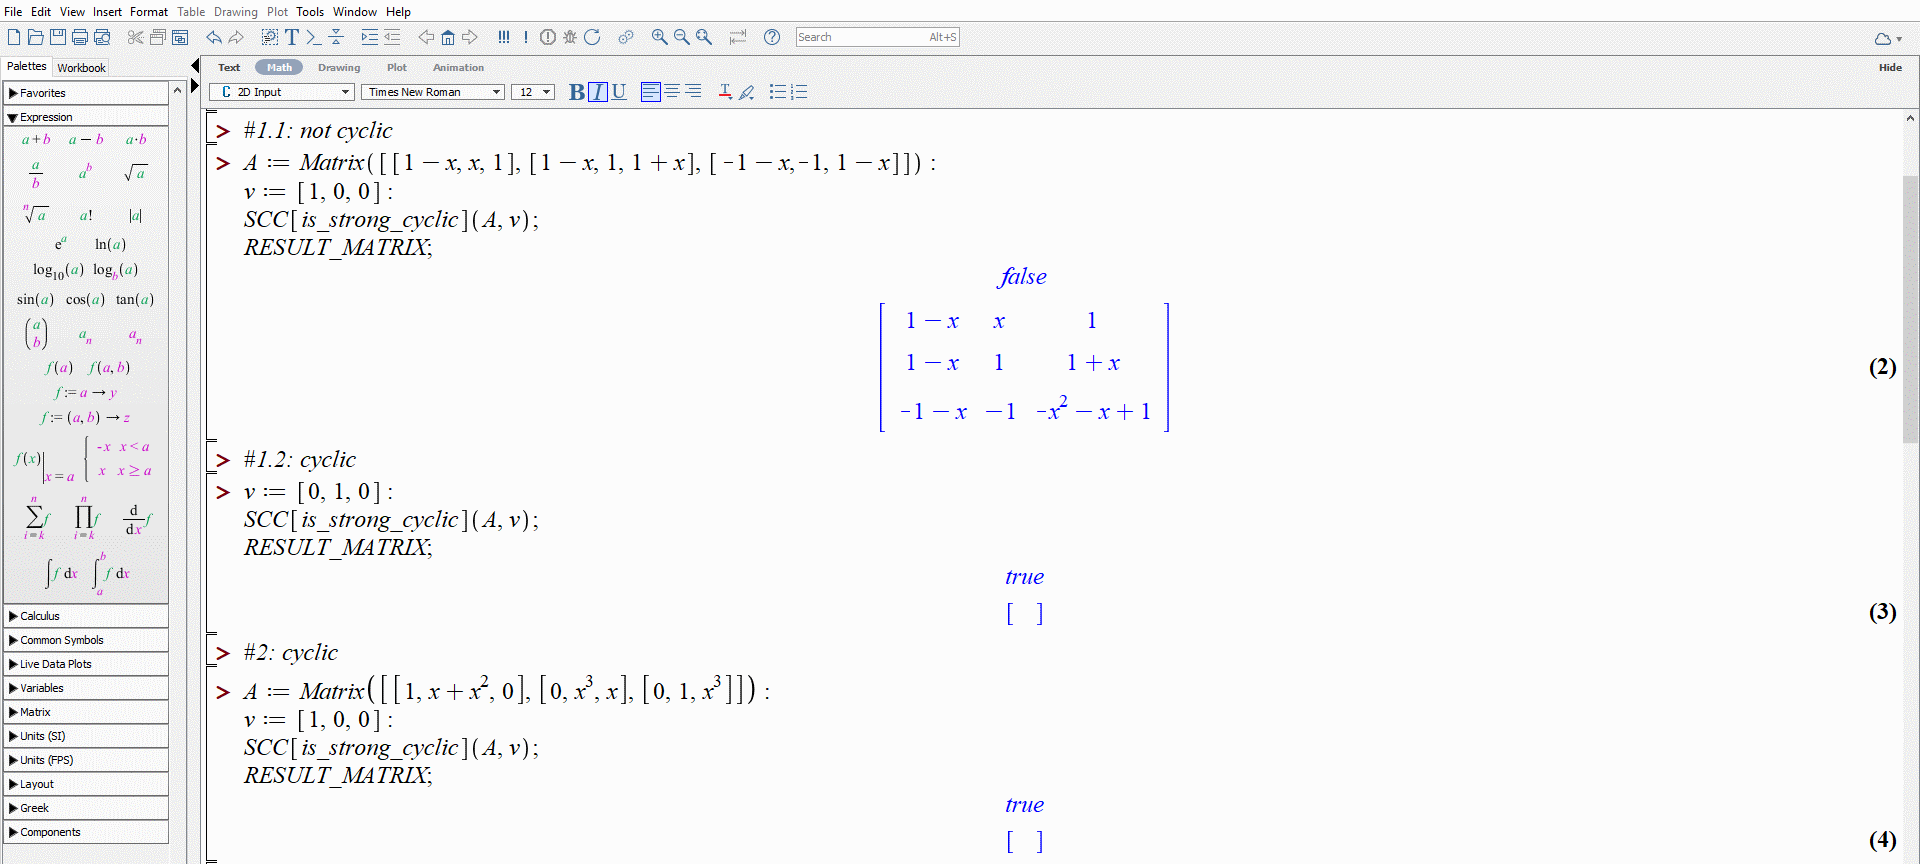
\includegraphics[scale=0.3]{pictures/maple_workarea.png}

    \small
    Рис. 7.1. Рабочая область в Мэйпл
\end{center}

Рабочая область состоит из~последовательных ячеек, содержащих обычный текст или математические выражения.
По команде пользователя все содержимое ячейки может быть выполнено, при~этом результаты вычисления появятся под~ячейкой.
Эти результаты могут быть использованы в~дальнейших расчетах.

Мэйпл предоставляет свой собственный язык программирования \cite{litMapleGuide2011, litMapleGuide2021},
который может быть использован для~реализации своих собственных процедур и структур данных.
Присутствуют все обычные элементы императивной парадигмы программирования:
циклы, присваивания, переменные, условные выражения, списки и пр.
Реализованные процедуры могут быть объединены в~\emph{пакет процедур}
для~дальнейшего использования в~своих работах в~Мэйпл.

\newpage

\subsection{Архитектура пакета}

Для удобства содержимое пакета было разбито на~4~файла, каждый из~которых выполняет свою функцию:

\begin{itemize}
    \item
        \verb|polynom.mm| "--- содержит базовые процедуры для~работы с~полиномами:
        \begin{itemize}
            \item
                \verb|max_degree| "--- определение максимальной степени~$x$ в~выражении;
            \item
                \verb|prolong| "--- построение продолжения многочлена указанным слагаемым.
        \end{itemize}
    \item
        \verb|cyclic.mm| "--- содержит базовые процедуры для~работы с~циклическими векторами:
        \begin{itemize}
            \item
                \verb|CV_dv| "--- построение матрицы производных вектора в~силу системы.
        \end{itemize}
    \item
        \verb|strong_cyclic.mm| "--- содержит реализацию основной процедуры \verb|is_strong_cyclic| проверки того,
        является~ли вектор сильно циклическим;
    \item
        \verb|strong_cyclicity_checking.mpl| "--- главный файл пакета, объединяющий все в~единое целое.
\end{itemize}

Далее приведено более подробное описание реализованных процедур.
Исходный код данных процедур приведен в \emph{Приложении А}.

\begin{itemize}
    \item
        Процедура для~определения степени многочлена:
        
        \verb|max_degree := proc(p)|

        Единственный ее параметр \verb|p| "--- выражение, имеющее вид многочлена от~$x$,
        которое может дополнительно содержать слагаемое вида~$O(x^t)$.
        Возвращает степень многочлена, которая затем будет использоваться при~построении продолжения данного многочлена.

    \item
        Процедура для построения продолжения многочлена:
        
        \verb|prolong := proc(p, coef, degree)|

        Принимает 3 параметра:
        \begin{itemize}
            \item
                \verb|q| "--- многочлен от~переменной~$x$;
            \item
                \verb|coef| "--- символьный или числовой коэффициент;
            \item
                \verb|degree| "--- степень, которой необходимо продолжить многочлен.
        \end{itemize}

        Процедура возвращает новый многочлен, являющийся продолжением многочлена~\verb|q(x)|.
        Продолжение получается добавлением к~многочлену нового слагаемого~$coef \cdot x^{degree}$.

    \item
        Процедура для~построения матрицы производных в~силу системы:
        
        \verb|CV_dv := proc(A, v, m)|
        
        \newpage
        Принимает 2 или 3 параметра:
        \begin{itemize}
            \item
                \verb|A| "--- квадратная матрица с коэффициентами, являющимися полиномами от~независимой переменной~$x$,
                элементы также могут содержать слагаемые вида~$O(x^t)$;
            \item
                \verb|v| "--- вектор с~коэффициентами, являющимися полиномами от~независимой переменной~$x$;
            \item
                \verb|m| "--- количество столбцов результирующей матрицы, которое нужно вычислить
                (значение по~умолчанию: размер матрицы~\verb|A|).
        \end{itemize}

        Данная процедура возвращает матрицу,
        столбцами которой являются $v$, $\diffVector$, $\diffVector[2]$, $\cdots$, $\diffVector[m-1]$.
        При $m=n$ эта матрица будет являться матрицей производных в~силу системы для~матрицы~\verb|A| и вектора~\verb|v|,
        которая может использоваться для~определения~того, является~ли вектор~\verb|v| циклическим.
\end{itemize}

Сам алгоритм проверки сильной цикличности вектора был реализован в~виде двух процедур:
\begin{itemize}
    \item
        \verb|is_strong_cyclic| "--- процедура, которую непосредственно вызывает пользователь;
        вызывает рекурсивную процедуру с~нужными параметрами;
    \item
        \verb|is_strong_cyclic_process| "--- рекурсивная процедура, выполняющая основные вычисления.
\end{itemize}

Более подробно про эти процедуры:
\begin{itemize}
    \item
        \verb|is_strong_cyclic := proc(A, v, max_recursion_depth)|

        Принимает 2 или 3 параметра:
        \begin{itemize}
            \item
                \verb|A| "--- квадратная матрица с коэффициентами, являющимися полиномами от~независимой переменной~$x$,
                элементы также могут содержать слагаемые вида~$O(x^t)$;
            \item
                \verb|v| "--- вектор с~коэффициентами, являющимися полиномами от~независимой переменной~$x$;
             \item
                \verb|max_recursion_depth| "--- целое число,
                ограничивающее допустимую глубину рекурсии при~построении опровергающего продолжения.
                Если не~задано, будет использовано значение по~умолчанию (см.~ниже).
        \end{itemize}

        Использование слагаемых вида~$O(x^t)$ в матрице \verb|A| позволяет указывать процедуре~то, какие степени многочленов
        представлены в~коэффициентах.
        Например, выражение $x + 4x^2 + O(x^5)$ следует интерпретировать как~многочлен 4-й степени,
        у~которого коэффициенты перед~3-й и 4-й степенью равны нулю.

        \newpage
        Возвращает одно~из~трех логических значений:
        \begin{itemize}
            \item
                \verb|false| "--- вектор не~является сильно циклическим;
                в переменной \verb|RESULT_MATRIX| (см. ниже) будет содержаться построенное опровергающее продолжение.
            \item
                \verb|true| "--- вектор является сильно циклическим.
             \item
                \verb|fail| "--- не~удалось получить ответ (уперлись в~максимально допустимую глубину рекурсии
                при~построении продолжения).
        \end{itemize}

    \item
        \verb|is_strong_cyclic_process := proc(A, v, steps_left, degree_matrix)|

        Принимает 4 параметра:
        \begin{itemize}
            \item
                \verb|A| "--- квадратная матрица с~коэффициентами, являющимися полиномами от~независимой переменной~$x$,
                элементы также могут содержать слагаемые вида~$O(x^t)$
            \item
                \verb|v| "--- вектор с~коэффициентами, являющимися полиномами от~независимой переменной~$x$
            \item
                \verb|steps_left| "--- целое число,
                указывающее максимально допустимую глубину рекурсии для~данного этапа.
            \item
                \verb|degree_matrix| "--- квадратная матрица того~же размера, что и~\verb|A|,
                содержит целые числа "--- степени многочленов в~соответствующих элементах матрицы~\verb|A|.
        \end{itemize}
\end{itemize}


Пользователь имеет доступ к~нескольким глобальным переменным, которые могут регулировать работу алгоритма:
\begin{itemize}
    \item
        \verb|MAX_RECURSION_DEPTH| "--- целое число, являющееся значением по~умолчанию для~максимально допустимой глубины рекурсии.
        По умолчанию равно~10.
    \item
        \verb|VERBOSE| "--- булевый флаг, при установке в~\verb|true| процедура будет подробно расписывать процесс вычислений.
        По умолчанию равно~\verb|false|.
    \item
        \verb|RESULT_MATRIX| "--- в~эту переменную будет записана матрица, являющаяся опровергающим продолжением,
        в~случае, когда удалось построить опровергающее продолжение.
\end{itemize}


\newpage
\subsection{Использование пакета StrongCyclicityChecking}

Реализация алгоритма доступна в виде набора процедур для~Мэйпл по~следующей ссылке:
\url{https://github.com/KingAArtur/strong-cyclicity-checking}.

На рис.~7.2 и 7.3 приведены примеры использования процедуры \verb|is_strong_cyclic|.


\begin{center}
    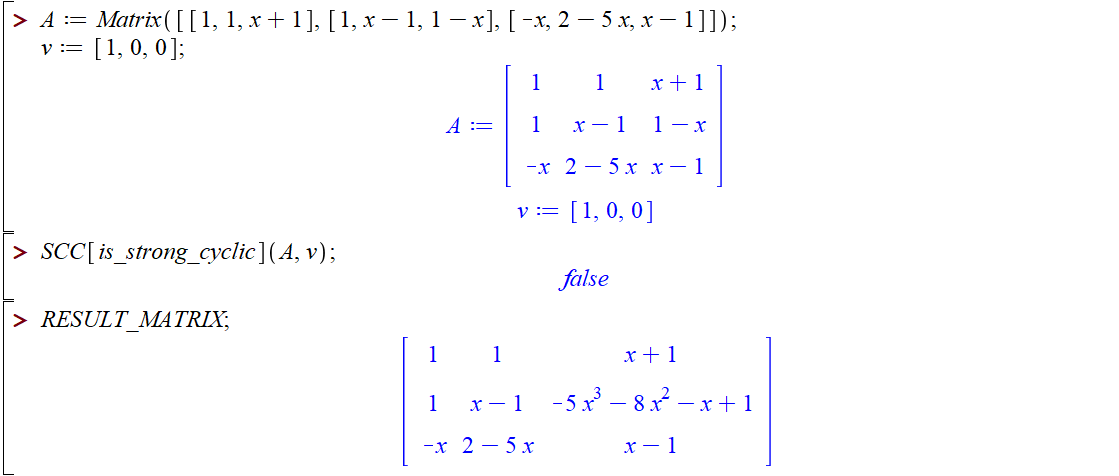
\includegraphics[scale=0.6]{pictures/maple_example4.png}

    \small
    Рис. 7.2. Пример работы процедуры для~не~сильно циклического вектора
\end{center}


\begin{center}
    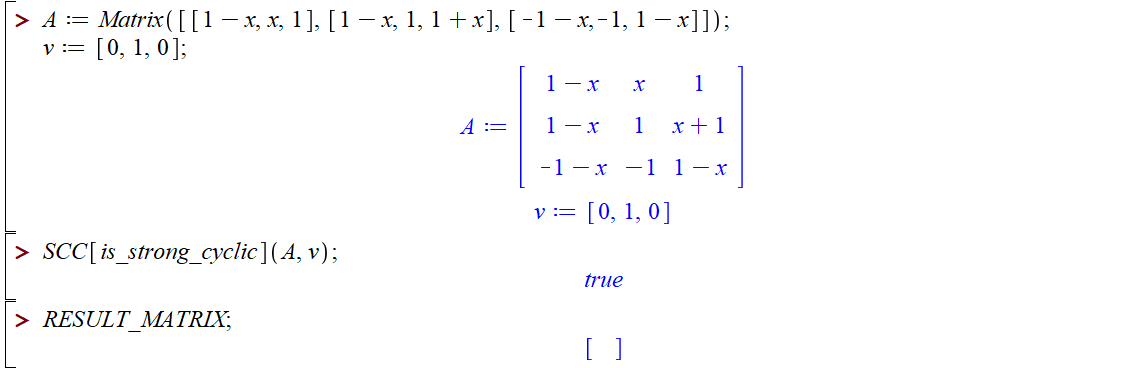
\includegraphics[scale=0.6]{pictures/maple_example1.png}

    \small
    Рис. 7.3. Пример работы процедуры для~сильно циклического вектора
\end{center}

Больше примеров можно найти там~же, где и исходный код:
\url{https://github.com/KingAArtur/strong-cyclicity-checking}.

% ============================== Заключение
\newpage
\section{Заключение}

В процессе данной работы были решены следующие задачи:

\begin{itemize}
	\item
		Доказан ряд утверждений о~сильно циклических векторах.
	\item
		Разработан частичный алгоритм проверки сильной цикличности вектора.
	\item
		Алгоритм реализован в~системе компьютерной алгебры Мэйпл и доступен на~GitHub:
		\url{https://github.com/KingAArtur/strong-cyclicity-checking}.
\end{itemize}

Следует выделить следующие возможные направления дальнейшей работы:

\begin{itemize}
	\item
		Построение опровергающего продолжения наверняка не~является единственным способом проверки сильной цикличности вектора,
        можно пытаться придумать другие подходы к~данной задаче.
	\item
		Интересна задача генерации сильно циклических векторов для~заданной усеченной системы.
	\item
		Можно задаться вопросом решения усеченных систем и нахождения информации о~решениях,
        инвариантной относительно возможных продолжений коэффициентов системы.
\end{itemize}


% ============================== Список литературы
\newpage
\section{Список литературы}

\begingroup
\renewcommand{\section}[2]{}

\begin{thebibliography}{10}

    \bibitem{litKovacic}
        R.\,C.~Churchill and J.~Kovacic.
        Differential algebra and related topics, 2000
    
    \bibitem{litAbramovResolvingSequences}
        Abramov~S.\,A., M.~Petkovsek, Ryabenko~A.\,A.
        Resolving Sequence of Operators for Linear Ordinary Differential and Difference Systems of Arbitrary Order~//
        Computational Mathematics and Mathematical Physics, 2016, Vol. 56, Issue. 5, P.\,894–910.
    
    \bibitem{litAbramovPowerSeries}
        Abramov~S.\,A., Barkatou~M.\,A.
        Computable Infinite Power Series in the Role of Coefficients of Linear Differential Systems~//
        Proc. of CASC’2014, 2014. P.\,1--12
    
    \bibitem{litVanDerPut}
        Marius van der Put, Michael F. Singer.
        Differential Galois Theory "--- USA, 2001

    \bibitem{litAbramovTruncatedSeries}
        Абрамов~С.\,А., Рябенко~А.\,А., Хмельнов~Д.\,Е.
        Линейные обыкновенные дифференциальные уравнения и усеченные ряды~//
        Журнал вычислительной математики и математической физики, 2019, том\,59, №\,10, с.\,1706--1717

    \bibitem{litAbramovScalarEquations}
        Абрамов~С.\,А., Рябенко~А.\,А., Хмельнов~Д.\,Е.
        Процедуры поиска усеченных решений линейных дифференциальных уравнений с бесконечными и усеченными степенными рядами в качестве коэффициентов~//
        Программирование, 2021, №2, с.\,56-65.

    \bibitem{litPanferov}
        Панфёров А. А.
        Сильно циклические векторы дифференциальных систем с полиномиальными коэффициентами~//
        Ломоносовские чтения-2020. "--- М.: М., 2020. "--- С.\,110--112.
    
    \bibitem{litMapleHelp}
        Maple Online Help "--- URL: \url{https://www.maplesoft.com/support/help/} (дата обращения 14.03.2023).

    \bibitem{litMapleGuide2011}
        Maple Programming Guide (2011)~//
        L. Bernardin, P. Chin, P. DeMarco и др. "---
        Maplesoft, a division of Waterloo Maple Inc. 2011.

    \bibitem{litMapleGuide2021}
        Maple Programming Guide "--- URL: \url{https://www.maplesoft.com/documentation_center/Maple2021/ProgrammingGuide.pdf} (дата обращения 15.03.2023).

\end{thebibliography}

\endgroup

% ============================== Приложение. Исходные коды функций
\newpage
\section*{Приложение А \\ Программный код основных функций}
\addcontentsline{toc}{section}{Приложение А. Программный код основных функций}


Функция для определения степени выражения, которое может содержать слагаемое вида $O(x^t)$
\begin{lstlisting}[basicstyle=\scriptsize]
max_degree := proc(p) :: integer;
    local result :: integer;
    
    if type(p, '`+`') or type(p, polynom) then
        # "polynom" - polynoms with or without "+", such as "x + 3x^3" or "4x^5"
        # "+" - polynoms with O(x^t) term, such as "2x + O(x^3)"
        if has(p, O) then
            # assuming that O(x^t) terms is max degree in the expression
            result := degree(op(select(has, p, O)), x) - 1;
        else
            if p = 0 then
                result := -1
            else
                result := degree(p, x)
            end if;
        end if;
    else
        # only O(x^t) term without any other terms, such as "O(x^4)"
        result := degree(op(p), x) - 1;
    end if;
    
    return result;
end proc:
\end{lstlisting}


\bigskip
Функция для построения матрицы производных вектора в силу системы
\begin{lstlisting}[basicstyle=\scriptsize]
CV_dv := proc(A, v, m)
    local n, i, j, k, W, AT, width;
    
    n := LinearAlgebra[RowDimension](A);
    if _npassed > 2 then
        width := m
    else
        width := n
    end if;
    
    AT := LinearAlgebra[Transpose](A);
    W := Matrix(n, width);
    for i from 1 to n do
        W[i, 1] := v[i]
    end do;
    
    for j from 2 to width do
        for i from 1 to n do
            W[i, j] := simplify(diff(W[i, j-1], x) + add(AT[i, k] * W[k, j-1], k = 1 .. n))
        end do
    end do;
    
    return(W);
end proc:
\end{lstlisting}


\newpage

Функция для построения продолжения многочлена
\begin{lstlisting}[basicstyle=\scriptsize]
prolong := proc(p :: polynom, coef, degree :: integer) :: polynom;
    local q;
    q := p + coef * x ^ degree;
    return q;
end proc:
\end{lstlisting}


\medskip
Процедура, запускающая алгоритм проверки сильной цикличности вектора
\begin{lstlisting}[basicstyle=\scriptsize]
is_strong_cyclic := proc(A :: Matrix, v :: list, max_recursion_depth :: integer) :: boolean;
    local actual_max_recursion_depth, n, degree_matrix, A_copied, i, j;
    
    if _npassed <= 2 then
        actual_max_recursion_depth := MAX_RECURSION_DEPTH
    else
        actual_max_recursion_depth := max_recursion_depth
    end if;
    
    show("=====");
    show("Starting calculations...");
    show("max_recursion_depth" = actual_max_recursion_depth);
    show("=====");
    
    n := LinearAlgebra[RowDimension](A);
    
    # calculating degrees for each element and removing O-notation
    degree_matrix := Matrix(n);
    A_copied := LinearAlgebra[Copy](A);
    for i from 1 to n do
        for j from 1 to n do
            degree_matrix[i, j] := max_degree(A_copied[i, j]);
            A_copied[i, j] := remove_o_notation(A_copied[i, j]);
        end do;
    end do;
    
    # clearing result matrix
    RESULT_MATRIX := Matrix():
    
    # calling recursive procedure
    return is_strong_cyclic_process(A_copied, v, actual_max_recursion_depth, degree_matrix);
end proc:
\end{lstlisting}


Рекурсивная часть алгоритма проверки сильной цикличности вектора
\begin{lstlisting}[basicstyle=\scriptsize]
is_strong_cyclic_process := proc(A :: Matrix, v :: list, steps_left :: integer, degree_matrix :: Matrix) :: boolean;
    local n, A_copied, degree_matrix_copied, CV, det, i, j, k, c, root, roots, solutions, failed, result;

    show("=====");
    show("depth" = steps_left);
    show(A);
    
    if steps_left = 0 then
        show(FAIL);
        return FAIL;
    end if;
    
    n := LinearAlgebra[RowDimension](A);
    A_copied := LinearAlgebra[Copy](A);
    degree_matrix_copied := LinearAlgebra[Copy](degree_matrix);
    
    # finding all 1-element prolongations that make tr(det) = 0
    solutions := [];
    for i from 1 to n do
        for j from 1 to n do
            A_copied[i, j] := A_copied[i, j] + c * x ^ (degree_matrix_copied[i, j] + 1);
            CV := CV_dv(A_copied, v);
            det := sort(collect(LinearAlgebra[Determinant](CV), x), [x]);
            
            roots := find_roots(tcoeff(det, x), c);
            show(A_copied);
            show(det);
            show(roots);
            
            # checking all found roots and appending them to the list
            for k from 1 to numelems(roots) do
                if roots[k] <> 0 then
                    if eval(det, c=roots[k]) = 0 then
                        # prolongation was found! => not strong cyclic
                        A_copied[i, j] := A[i, j] +
                            roots[k] * x ^ (degree_matrix_copied[i, j] + 1);
                        RESULT_MATRIX := A_copied;
                        show("not cyclic!");
                        return false;
                    end if;
                    solutions := [op(solutions), [i, j, roots[k]]];
                end if;
            end do;
            
            # discarding changes for this element
            A_copied[i, j] := A[i, j];
        end do;
    end do;
    
    # recursively applying to all collected prolongations
    failed := false;
    for k from 1 to numelems(solutions) do
        i, j, root := solutions[k, 1], solutions[k, 2], solutions[k, 3];
        
        A_copied[i, j] := A_copied[i, j] + root * x ^ (degree_matrix_copied[i, j] + 1);
        degree_matrix_copied[i, j] := degree_matrix_copied[i, j] + 1;
        
        result := is_strong_cyclic_process(A_copied, v, steps_left-1, degree_matrix_copied);
        degree_matrix_copied[i, j] := degree_matrix[i, j];
        A_copied[i, j] := A[i, j];
        
        if result = false then
            show("not cyclic!");
            return false;
        end if;
        if result = FAIL then
            failed := true;
        end if;
    end do;
    
    if failed then
        show("FAIL");
        return FAIL;
    else
        show("yes, strong cyclic!");
        return true;
    end if;
end proc:

\end{lstlisting}



\end{document}